\chapter{Revisão Bibliográfica}\label{chap:revisao}

\section{Considerações Iniciais}

% A literatura em redução de dimensionalidade é extensa e os métodos desenvolvidos apresentam grande diversidade em relação a aspectos matemáticos e computacionais. Buscando uma melhor contextualização, esta seção aborda apenas trabalhos que buscam de alguma forma utilizar representações visuais para a execução desta tarefa.

Os trabalhos do atual estado da arte que mais se assemelham ao o aqui proposto aparecem sobre o nome de métodos de redução de dimensionalidade. 
A redução de dimensionalidade é o processo realizado para se representar dados de alta dimensionalidade em um espaço de menor dimensionalidade, onde, idealmente, o espaço reduzido corresponde à dimensionalidade intrínseca dos dados. 
Por sua vez, a dimensionalidade intrínseca dos dados é o número mínimo de parâmetros necessários para descrever as propriedades dos dados~\cite{Fukunaga1990}.

Dentre os propósitos da redução de dimensionalidade, os principais são a melhoria na eficiência dos métodos que operam sobre os dados e a redução do custo computacional desses métodos.  
\citeauthor{Konig2000}~\cite{Konig2000}, por exemplo, apresenta melhorias na precisão de sistemas de classificação e no desempenho de sistemas de reconhecimento automático ao preceder os procedimentos com o processo de redução de dimensionalidade. 
Até mesmo outros benefícios não tão diretos podem ser alcançados por meio do uso de técnicas de redução. 
Trata-se do caso do mesmo trabalho apresentado por \citeauthor{Konig2000}, onde métodos de redução de dimensionalidade são utilizados para reduzir a complexidade de designs de circuitos integrados, resultando em uma redução na área e no consumo de energia dos circuitos.

Uma terceira utilidade para os métodos de redução de dimensionalidade é viabilizar a construção de representações visuais de dados multidimensionais~\footnote{No contexto de visualização computacional, conjuntos de dados multidimensionais são aqueles com mais do que três atributos.}, permitindo que sejam mapeados em um espaço bidimensional (tela computador).
Representações visuais dos dados são cruciais para a análise exploratória de dados, principalmente para investigações iniciais dos dados, onde ainda não se conhece as propriedades dos dados~\cite{Kaski2011}. 

A literatura em redução de dimensionalidade é extensa e os métodos desenvolvidos apresentam grande diversidade em relação a aspectos matemáticos e computacionais. 
Buscando uma melhor organização, este capítulo foi dividido em duas seções. 
A primeira busca descrever sucintamente os métodos automáticos e apresentar suas limitações, principalmente evidenciar que a falta da participação do usuário no processo faz com que muitas vezes os resultados obtidos não sejam facilmente compreendidos. 
A segunda seção apresenta os métodos que permitem que o usuário participe do processo de redução de dimensionalidade por meio da interação com representações visuais. 
Ao longo da segunda seção discute-se que apesar dos métodos interativos se mostrarem como uma interessante alternativa, os mecanismos de interação propostos apresentam grandes limitações. 
Nas considerações finais deste capítulo, resume-se as principais limitações dos métodos interativos. 

\section{Redução de Dimensionalidade Automática}

A redução de dimensionalidade automática pode ser realizada seguindo duas abordagens. 
A primeira transforma os atributos de entrada em um novo conjunto de dimensões que busca conservar certas propriedades ou relacionamentos do conjunto original. 
Por extrair um novo conjunto de atributos a partir dos dados originais, esta abordagem recebe o nome de extração de características (\emph{feature extraction}).
Já a segunda abordagem busca selecionar quais dos atributos do conjunto de dados são realmente relevantes para a análise segundo algum critério. 
Como os dados não são modificados, esta segunda abordagem é chamada de seleção de características (\emph{feature selection}).

\subsection{Extração de Características}

O problema de extração de características pode ser descrito da seguinte forma: 
Dado um conjunto de dados representado por uma matriz $\textbf{X}$ composta por $n$ vetores $\textbf{x}_i~(i \in \{1,2,...,n\})$ $m-$dimensionais, deseja-se encontrar uma transformação $t: \textbf{X} \rightarrow \textbf{Y}$, onde $\textbf{Y}$ trata-se de uma matriz composta por $n$ vetores $\textbf{y}_i~(i \in \{1,2,...n\}$ de dimensionalidade $p$ ($p < m$). 
Normalmente $p \ll m$ e, idealmente, $p$ equivale à dimensionalidade intrínseca dos dados, fazendo com que $t$ mantenha em $\textbf{Y}$ o máximo das propriedades de $\textbf{X}$ quanto for possível. 

Como apresentado por~\citeauthor{Maaten2009}~\cite{Maaten2009} e ilustrado na Figura~\ref{fig:fex}, existe uma grande variedade de métodos de extração de características. Não é intuito desta subseção detalhar cada uma dessas técnicas e levantar suas limitações particulares, mas sim ilustrar a limitação que todas apresentam em comum de retornar resultados pouco intuitivos para o usuário e impedi-lo de interagir com os dados. Para este fim, o método de análise de componentes principais (PCA) será utilizado como base para os exemplos.

\begin{figure}[h!]
    \centering
    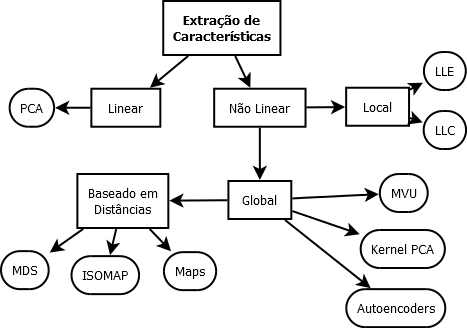
\includegraphics[width=10cm]{images/fex.png}
    \caption[Principais Métodos de Extração de Características.]{Principais métodos de extração de características, adaptado de \cite{Maaten2009}.}
    \label{fig:fex}
\end{figure}

% LER OS PAPERS DE RED DIM PARA INSPIRAÇÃO E REFERÊNCIAS.

% Existem três principais abordagens para se reduzir a dimensionalidade dos conjuntos de dados a partir da combinação dos atributos. Análise de Componentes Principais (\textit{Principal Component Analysis)}~ ou simplesmente PCA, realiza combinações lineares sobre os atributos de modo que o novo espaço agregue a maior parte da variância dos dados. Para análises onde relações não lineares devem ser consideradas, \textit{Multimensional Scaling} (MDS) é uma alternativa interessante, pois trata-se de um algoritmo de otimização iterativo não linear, que busca minimizar as distâncias entre os elementos no espaço projetado e no espaço original. A área de aprendizado de máquina contribuiu com o método não supervisionado \textit{Self Organizing Maps} (SOM) para transformar conjuntos de dados em mapas bidimensionais.

% Sem dúvida a técnica mais importante é PCA

\subsection{Seleção de Características} 

O objetivo dos métodos de seleção de características é encontrar o subconjunto  dos atributos de entrada mais adequado para a aplicação em estudo. 
Assim, busca-se identificar e eliminar atributos redundantes~\cite{Kohavi1997} ou que não apresentem correlação com o fenómeno investigado~\cite{Nilsson2007}. 
Por exemplo, em tarefas de classificação supervisionada, pode-se determinar a importância de um atributo avaliando sua correlação com o atributo classe. 

O funcionamento desses métodos consiste em realizar uma busca sobre subconjuntos candidatos e tomar como resultado o subconjunto que apresenta melhor avaliação de acordo com uma função pré estabelecida. 
O caso completo trata-se da avaliação de $2^m$ subconjuntos (todas as combinações possíveis), onde $m$ corresponde ao número de atributos do conjunto de entrada. 
Tal situação equivale a um problema $np$-completo, consequentemente para grandes conjuntos de dados a solução ótima não pode ser obtida em tempo fazível, exigindo assim a adoção de alguma eurística. 

As diferentes eurísticas que podem ser adotadas constituem a literatura em seleção de características. A Figura ilustra os principais métodos.

Em comparação aos métodos de extração, os métodos de seleção apresentam a vantagem de que o resultado obtido é mais intuitivo ao usuário, pois se trata de um subconjunto do conjunto de entrada. 
Assim, se o usuário tem certo conhecimento sobre o conjunto de entrada, então será capaz de compreender os resultados obtidos.
No entanto, eles compartilham a mesma natureza caixa-preta que priva o usuário de qualquer interação durante o processo de redução, impedindo que o usuário contribua com seu conhecimento sobre o domínio e compreenda quais características dos seus dados foram responsáveis por aquele resultado.

\section{Redução de Dimensionalidade Interativa}

\subsection{Value and Relation Display}\label{sec:var}

A técnica VaR (Value and Relation)~\cite{Yang2004} une os conceitos de MDS e glifos para representar as dependências entre as dimensões de uma base de dados. Como mostra a Figura~\ref{fig:var1}, cada glifo representa uma dimensão e de acordo com seus posicionamentos no plano o usuário pode compreender quais dimensões se relacionam entre si. O usuário é capaz de construir espaços dimensionais reduzidos que conservam certas características dos dados por meio de seleções sobre os dados ou pelo uso de um método automático que a partir de uma dimensão de referência e um \emph{threshold} definido pelo usuário retorna as dimensões mais semelhantes.

\begin{figure}[h!]
  \centering
  \begin{subfigure}[b]{0.5\textwidth}
    \centering
    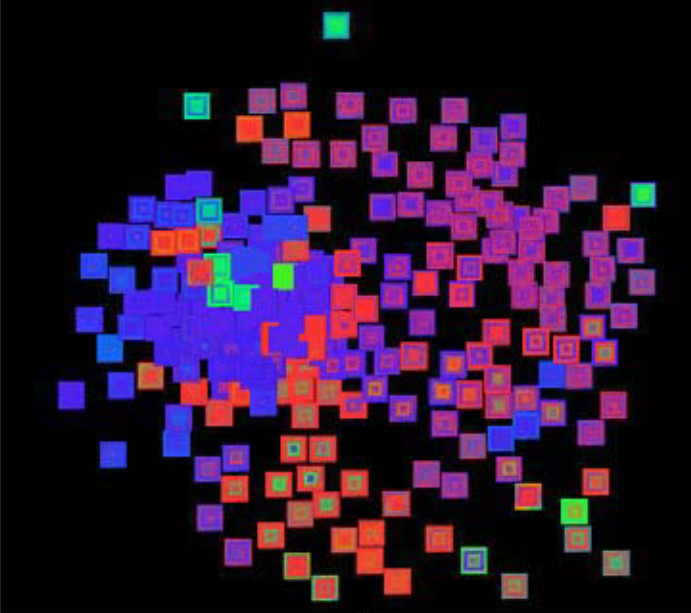
\includegraphics[width=\textwidth]{images/var1.png}
    \caption{}
    \label{fig:var1}
  \end{subfigure}%
  ~ %add desired spacing between images, e. g. ~, \quad, \qquad etc.
  \begin{subfigure}[b]{0.475\textwidth}
    \centering
    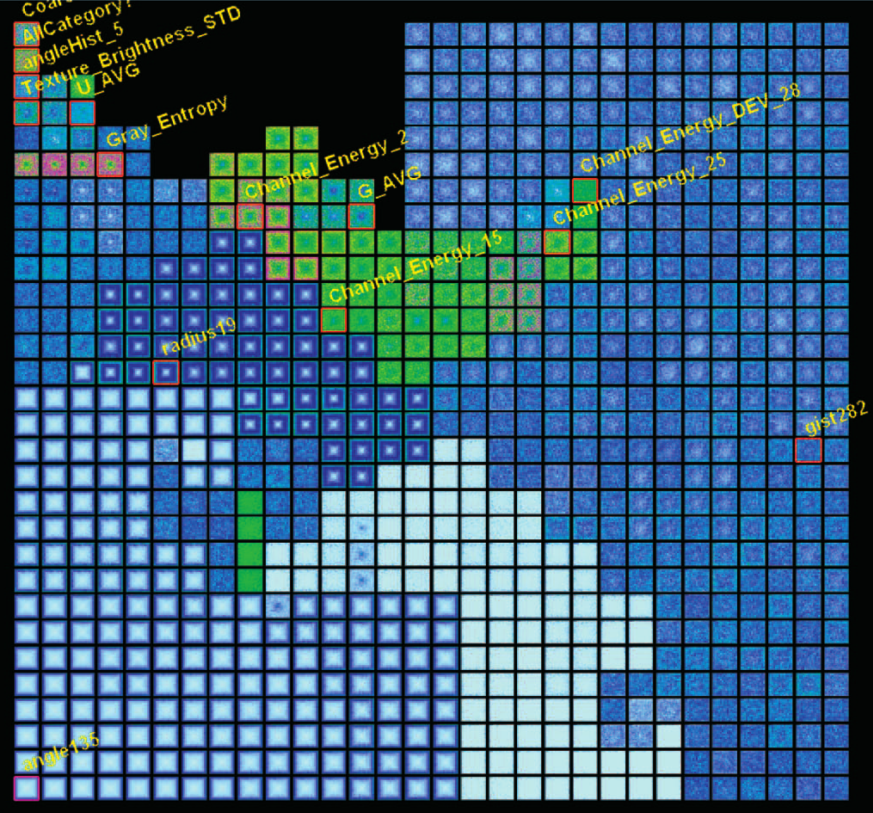
\includegraphics[width=\textwidth]{images/var2.png}
    \caption{}
    \label{fig:var2}
  \end{subfigure}
  \caption[VaR: Value and Relation]{(a) Exemplo da técnica VaR para um conjunto de $50.000$ itens e $361$ dimensões. Cada dimensão é representada por um glifo e seus posicionamentos refletem a similaridade entre as dimensões, de modo que glifos que se encontram próximos indicam atributos que apresentam alguma relação entre si. É possível notar certas sobreposições entre os glifos, condição que pode dificultar as análises realizadas pelo usuário. (b) Exemplo de representação alternativa proposta como extensão da técnica VaR para um conjunto de 11.413 itens e 838 dimensões. O principal objetivo da representação é evitar a sobreposições de glifos ocorrente na versão anterior da técnica.}
\end{figure}

O procedimento para a construção desta visualização inicia pela construção de uma matriz de distâncias que é responsável por capturar os relacionamentos entre pares de dimensões do conjunto de dados (como a correlação). Sobre esta matriz de distâncias aplica-se uma técnica de MDS para mapear cada dimensão em uma posição de um espaço bidimensional. Finalmente, cria-se um glifo orientado a pixels para cada dimensão que será utilizado para representar cada dimensão no plano.

% Esta etapa é comum à maioria dos trabalhos aqui discutidos e devido à sua importância para os métodos, será discutida com mais detalhes na Seção~\ref{sec:sim-dim}. 

Observando a Figura~\ref{fig:var1} é possível notar que o uso de glifos faz com que ocorram sobreposições, pois cada glifo requer um espaço relativamente grande para que seja observado adequadamente. As sobreposições dificultam as análises de regiões de interesse e podem fazer com que o usuário alcance conclusões inválidas, devido a oclusão de algum elemento importante. Buscando tratar este problema~\citeauthor{Yang2007} desenvolveram a extensão~\cite{Yang2007} ilustrada na Figura~\ref{fig:var2} para a técnica VaR, onde apresentaram alternativas para a projeção de glifos no plano. No entanto, diferentemente das projeções, as alternativas propostas não são capazes de transmitir os relacionamentos entre as dimensões tão bem quanto o resultado obtido pelo MDS.

A representação explícita das dimensões do conjunto de dados serve como inspiração para este trabalho de mestrado. Já o uso de glifos orientado a pixels se mostrou inadequado para situações com um elevado número de elementos, causando indesejadas sobreposições entre elementos. Um outro aspecto importante que os próprios autores mencionam em relação ao uso deste tipo de  glifos é que os usuários têm dificuldade em comparar glifos que se encontram afastados entre si. 

Uma etapa fundamental da técnica VaR que merece uma maior atenção é o método utilizado para a criação da matriz de distâncias. Os autores desenvolveram um novo método para cálculo da correlação entre dimensões que busca encontrar a maior discriminação entre os atributos. A seguir apresenta-se uma breve  descrição deste método:

\begin{enumerate}
   
    \item Dado um conjunto de dados com $m$ dimensões; 
    \item Normaliza-se os valores em respeito às colunas (invariância contra escala e translação);
    \item Para cada par de dimensões $Par(i,j)$ com $1 \leq i \leq m$ e $i < j \leq m$, constrói-se um histograma da diferença entre os valores $Hist(i,j)$. O número de \emph{bins} (classes) do histograma $numBins$ é uma constante definida pelo usuário;
    \item Para $k = 1$ até $numBins$ calcula-se $Var_k$:
    \begin{enumerate}
        \item Constrói-se a matriz $M_k$. A posição $M_k(i,j)$ da matriz será dada pelo valor $1$ subtraído da razão entre a população contida em $k-$classes mais frequentes de $Hist(i,j)$ e o total de elementos;
        \item $Var_k$ corresponde à variância dos elementos não diagonais da matriz;
    \end{enumerate}
\item Retorna-se $M_k$ que apresenta maior $Var_k$.

\end{enumerate}

Este método proposto foi comparado à Distância Euclidiana entre os elementos e mostrou-se que o novo método apresenta um aumento na discriminação entre os atributos de $45\%$ a $95\%$ maior. Ou seja, utilizando este método, os autores conseguiram separar melhor dimensões diferentes e agrupar melhor as que apresentam certa semelhança. No entanto, não foram realizadas comparações com outras medidas de correlação entre variáveis bem estabelecidas na  literatura (para uma melhor discussão sobre essas medidas favor consultar a Subseção~\ref{ss:sim}. Apesar dos autores mencionarem que o cálculo de uma medida de correlação não está vinculado ao processo da técnica de visualização, trata-se de uma etapa diretamente relacionada com a projeção dos dados, consequentemente está fortemente atrelada à qualidade do \emph{layout} apresentado.

\subsection{Brushing Dimensions}

A exploração das relações entre as dimensões não precisa estar vinculada somente a representações visuais dos atributos do conjunto de dados. \citeauthor{Turkay2011}~\cite{Turkay2011} propuseram um método de múltiplas visões que permite que o usuário interaja tanto com as dimensões quanto com os itens da base de dados. O principal mecanismo de interação é a seleção que se reflete em outras visões e permite que se visualize, por exemplo, as dimensões que melhor representam subconjuntos dos dados. Uma das limitações deste trabalho é falta de medidas que consideram pares de dimensões, como medidas de correlação, o que dificulta a observação de dependências entre os atributos.  

\section{Considerações Finais}

% Faço um resumo das limitações dos trabalhos apresentados ou de como eles podem ser importantes para o meu trabalho.

% VaR não faz redução propriamente dita.

% VaR não apresenta mecanismos adequados que facilitem a tarefa de redução de dimensionalidade.

% Métodos de coordenação tem sido muito utilizados, mas eles não se preocupam em manter a mesma metáfora visual.

% Menciono que as novas abordagens visuais apresentam certas limitações:

% 1. Cálculo da medida de similaridade (falta uma fundamentação teórica)
% 2. Mecanismos de interação inadequados (muitos utilizam sliders e exigem thresholds)
% 3. Carência de certos mecanismos de interação (nenhum propõe "arrastar dimensões", somente  selecionar e no máximo combiná-las) 
% 4. Sobrecarga sistema cognitivo do usuário (density pixels, variedade de metáforas visuais)

% "No entanto. poucas fornecem mecanismos de interação adequados, etc."

% Our main conclusion is that the focus of the research community should shift towards        nonlocal techniques for dimensionality reduction with objective functions that can be         optimized well in practice (such as PCA, Kernel PCA, and autoencoders).

